\documentclass[12pt]{article}
\usepackage{fourier}
\usepackage{listings}
\usepackage[utf8]{inputenc}
\usepackage{calc}
\usepackage{graphicx}
\usepackage{amsmath}
\usepackage{float}
\usepackage{amsfonts}
\usepackage{xcolor}
\usepackage{amsthm}
\usepackage{amssymb}
\usepackage{ragged2e}
\usepackage{flafter}
\usepackage{multirow}
\usepackage{geometry}
\usepackage{tabularx}
\usepackage{booktabs}
\usepackage{tabularray}
\usepackage{fancyvrb}
\usepackage{setspace}
\usepackage{hyperref}
\usepackage{subcaption}
\usepackage{wrapfig}

\geometry{
    textheight=9in,
    textwidth=5.5in,
    top=0.6in,
    headheight=12pt,
    headsep=25pt,
    footskip=30pt,
    left=0.6in,
    right=0.6in
}

\setstretch{1}
\setlength{\parindent}{0pt}

\begin{document}

\section*{Executive Summary}
Our main goal of this project is to investigate the possible causes of a patient experiencing a cardiac event. For the model selection process, we included: age, BMI, diabetes status, education, ethnic, gender, sleep hour, smoking status, and the interaction between gender and education. We utilized backward selection using AIC and BIC to pick the best logistic model for predicting cardiac event. The analysis revealed that individuals who identify as Black and smoke face a higher risk of experiencing a cardiac event, controlling for all other predictors. While marginally less so, we also found that older age and higher BMI were associated with an increased risk of cardiac events. 

\section*{Introduction}
Cardiac events (heart diseases) are the leading cause of death for people in the United States. They may be “silent” and not diagnosed until a person experiences signs or symptoms of heart attack or heart failure. Researches have shown that several medical conditions and lifestyle choices can put people at a higher risk for heart diseases. The dataset used in this study was collected from 1910 individuals during the time period spanning from 2017 to 2020. It includes measures of health such as sleep hours, diabetes status, smoking status, and BMI. The dataset also includes demographic data such as age, gender, race, and education. \\

The goal of this study is to determine which combination of predictor variables leads to the highest probability of developing a cardiac disease. We are particularly interested in the effect of nightly sleep on the development of cardiac disease. By unraveling these associations, we hope to contribute valuable insights into preventive strategies for individuals at risk. Although demographic factors cannot be controlled, individuals can take initiative to reduce their risk of cardiac events by controlling their lifestyle. The results from this study will inform people on the risk factors that they can control for. Health professionals can also utilize this information to identify individuals at risk and provide tailored interventions. \\

Before analyzing our data, we spent some time checking and cleaning it. First of all, we removed two columns (X and seqn) that served for identification purposes. We also ran a summary of statistics on the dataset to get an overview of all the variables. We then found out that there are four variables (sleep hour, diabetes, smoker, and bmi) with missing values (NA). There are also some categorical variables with “Don’t Know” and “Refuse to Answer”  categories, and we treated them as missing values. We then ran linear regression to predict the missing values for sleep hour and bmi. However, the regression models had poor performance (very low $R^2$ values), so we used the median values to replace the missing values. For smoker and diabetes, we ran logistic regression to predict the missing values. \\

After handling the missing values, we utilized the splicing plots and mosaic plots to classify variable types (categorical or numerical) and re-code the categorical variables. The splicing plots also help us determine whether we need to transform the numerical variable before model fitting. We ran a splicing plot for each of the numerical variables to determine variable classification and transformation. For the categorical variables, we ran mosaic plots and the trend test to determine if we needed to re-code them.\\

The next step was the two-way analysis, which evaluated the association between the outcome and each predictor. We ran a chi-square test of association on all the categorical predictors, noting the ones that are significant. For the numerical predictors, we ran a likelihood ratio test on each of them to determine their significance. 
As part of the model consideration process, we also looked into the interaction terms through interaction plots and likelihood ratio tests. These plots contained all the possible combinations of predictors. Included in our R code, we automated likelihood ratio tests on all possible combinations of predictors and their interaction terms. We filtered significant interaction terms to have a p-values less than 0.01. \\

As for model selection, we used AIC, BIC, and backward selection to curate our best model. After we picked our best model, we conducted the goodness-of-fit test to evaluate our model. We also created a ROC curve plot, classification table and probability plot to evaluate the overall fitness.\\

% After we identified the significant predictors and interaction terms, we moved on to model selection. We decided to use the stepwise backward selection to pick our best model. We ran the step function in R using both AIC and BIC as the evaluation criteria. Ideally, we want to choose the model with the lowest AIC, but we need to turn to BIC if there are two models with very close AIC values (less than 2). After we picked our best model, we conducted the goodness-of-fit test to evaluate our model. We also created a classification table and ROC curve to evaluate the overall fitness of our model.\\

\section*{Description of Subjects}
\subsection*{{Data Checking \& Handling Missing Values}}

The dataset initially contained 11 columns and 1910 rows. Each row in the data corresponds to an individual, uniquely identified by the “X” and “seqn” columns. The response variable for this dataset is “event”, an indicator variable with 1 corresponding to the presence of a cardiac event and 0 corresponding to the absence of the cardiac event. In addition to the response and identifier columns, the dataset includes eight variables: gender, age, ethnic (ethnic1), sleep hour (sleep.hrs), education (educ), diabetes, smoker, and bmi. Since the missing values composed of a significant portion of our data (approximately 14\% of the entire dataset), we decided to run regressions to predict these missing values.\\

\begin{wrapfigure}{l}{0.5\textwidth}
    \centering
    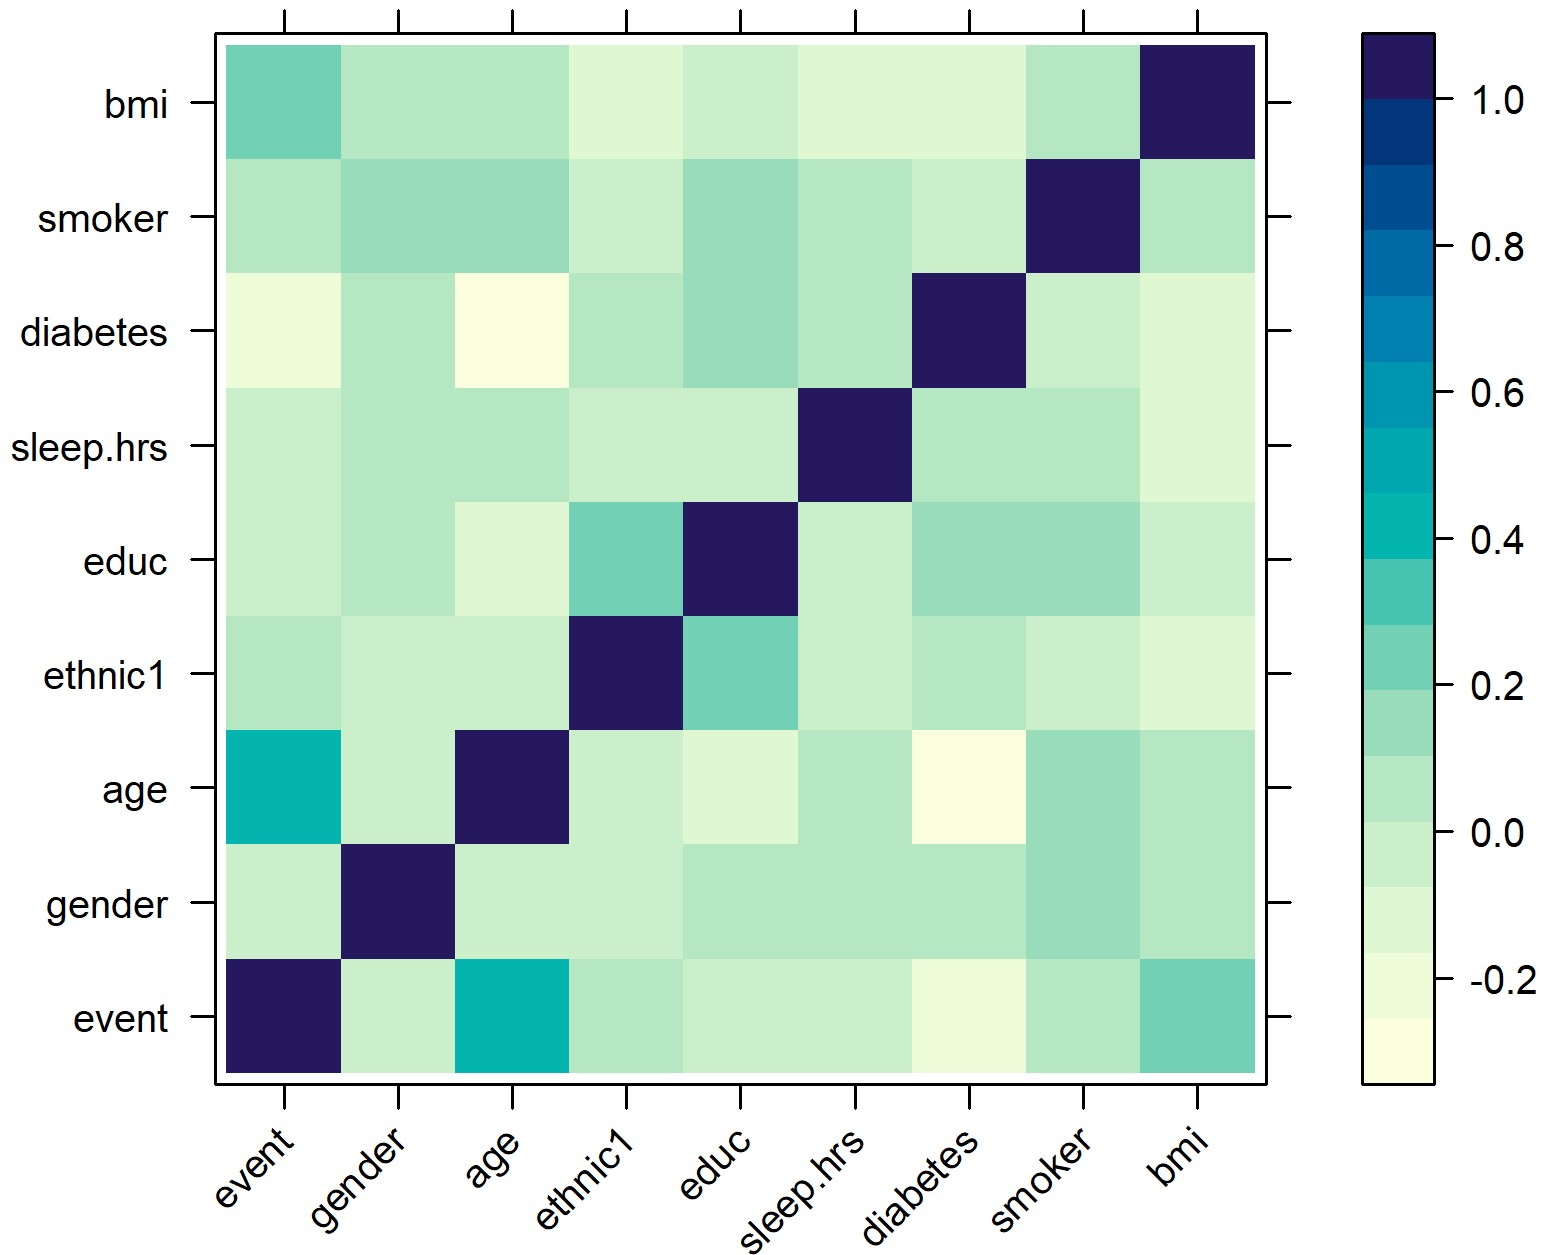
\includegraphics[width=0.5\textwidth]{Img/levelplot.jpg}
    \caption{Correlation table level plot}
\end{wrapfigure}

Before processing the variables, we first used the summary function in R to obtain an overview of all the variables. We found out that there are four variables (sleep hour, diabetes, smoker, and bmi) with missing values (NA). Furthermore, categorical variables like educ, diabetes, and smoker have values belonging to the “Don’t Know” and “Refuse to Answer” categories. We decided to treat these values as missing values. The educ variable only has one row with “Don’t Know” value and no other NA values, so we simply removed this record. For the other missing values, we decided the best approach would be to employ regressions to predict these missing values. Additionally, we built a correlation matrix and turned it into a more intuitive level plot (Figure 1) as below to help us determine the predictors that we use in our regression models, more specifically, for each variable, we look at the corresponding row or column to find the darkest grids to get the most correlated variables (except for event and itself).


%\begin{figure}[!htbp]
%\centering
%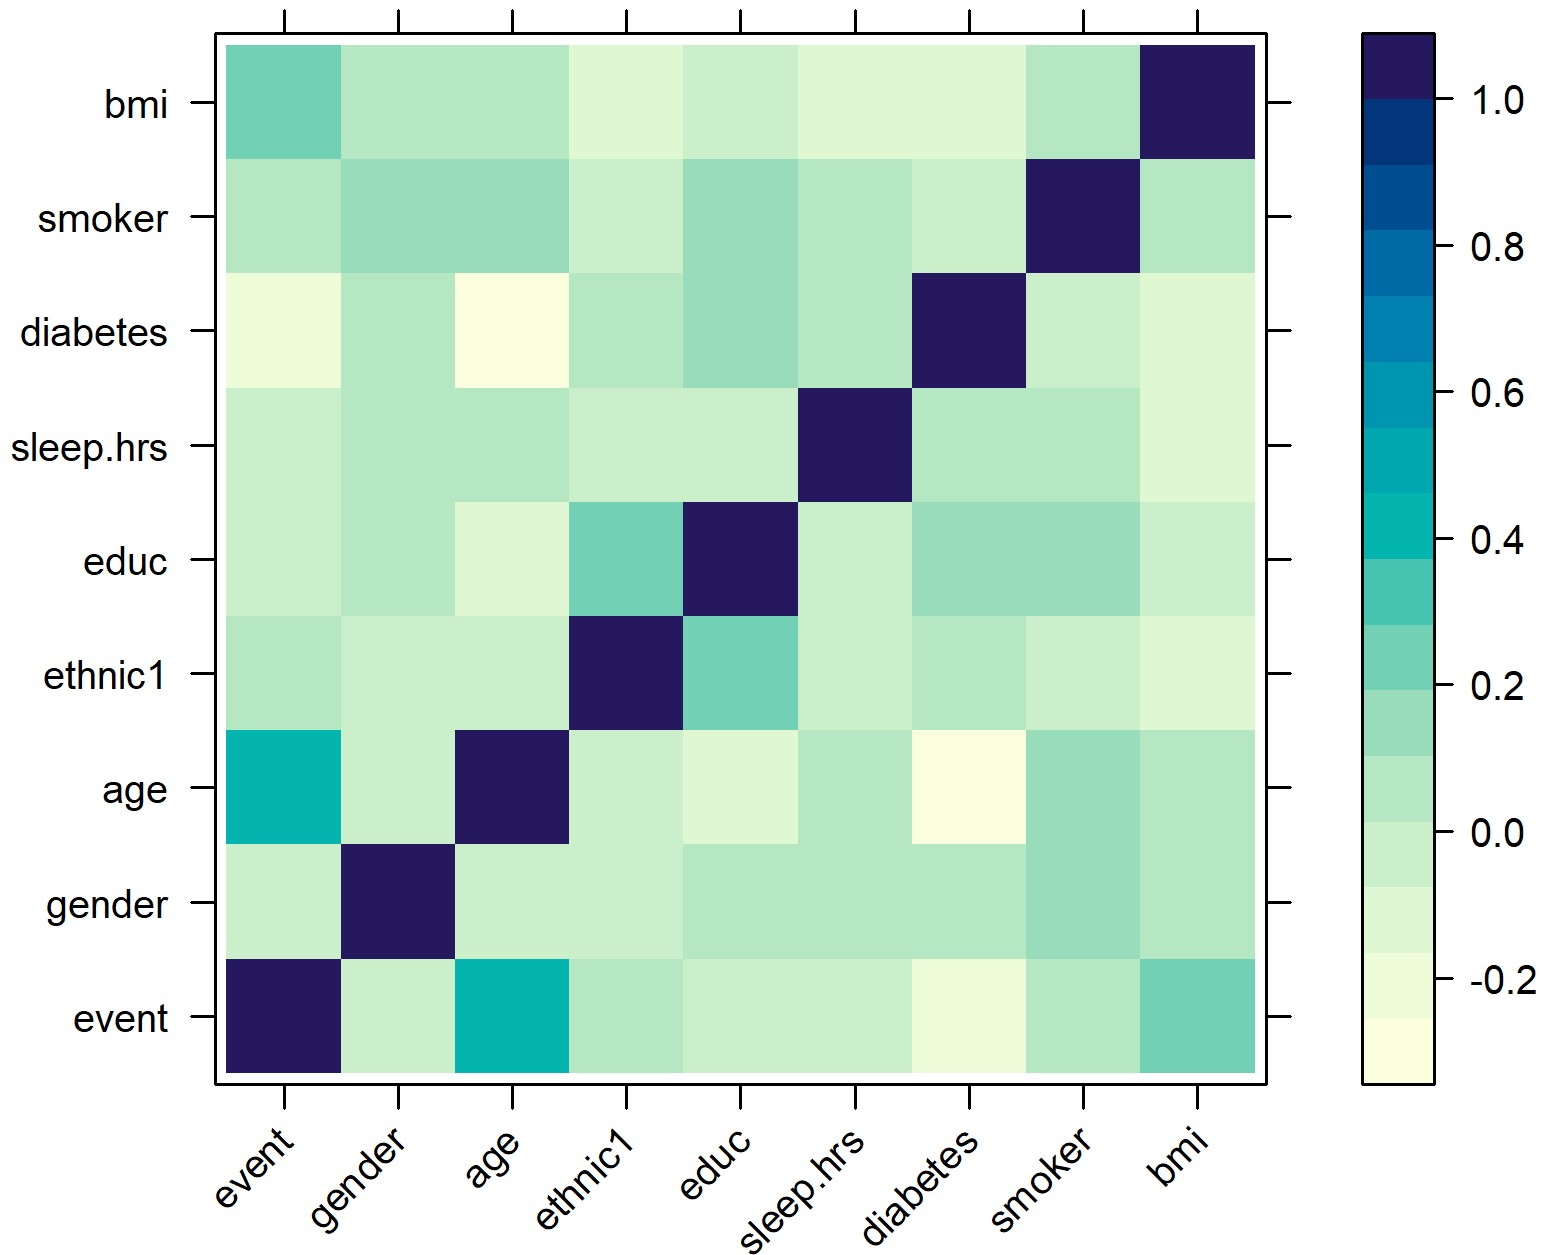
\includegraphics[width=0.4\linewidth]{Img/levelplot.jpg}
%\caption{Correlation table level plot}
%\end{figure}


% \textbf{\textit{Handling Missing Values: diabetes}}

\subsubsection*{{{Handling Missing Values: }}\protect\Verb+diabetes+}

The diabetes variable has one “Don’t Know” value, but it has many NA values. However, the issue we are facing is that the variable has three categories. The trend test we ran shows that diabetes has a linear association with cardiac events. The mosaic plot for diabetes also shows that each category has distinct odds, so we decided to keep the three categories. Since multiple logistic regression for ordinal categorical variables is out of the scope of this study, we decided to remove all the rows with missing diabetes value (about 3.8\% of the entire dataset).

% \textbf{\textit{Handling Missing Values: smoker}}
\subsubsection*{{{Handling Missing Values: }}\protect\Verb+smoker+}

The smoker variable has a total of 147 missing values. It has only two categories, so we can utilize a logistic regression to predict the missing values. In the model, we used gender, education, and age to predict tobacco use.

% \textbf{\textit{Handling Missing Values: sleep.hrs}}
\subsubsection*{{{Handling Missing Values: }}\protect\Verb+sleep.hrs+}

The sleep variable has a total of 13 missing values. Since it is a numerical variable, we used multiple linear regression models to predict the missing values. With the aid of correlation matrix, we tried two different models to predict sleep hours. The final model has a very low $R^2$ value, which is around 0.011. Due to the model’s poor performance, we used the median of sleep hours (7.5) to replace all the missing values.

% \textbf{\textit{Handling Missing Values: bmi}}
\subsubsection*{{{Handling Missing Values: }}\protect\Verb+bmi+}

The BMI variable has a total of 46 missing values. We also tried to use linear regression to predict the missing values, but the model also has poor performance ($R^2 = 0.025$). Thus, we used the median BMI, which is 30.48, to replace all the missing values.

\begin{table}[h]
\centering
\caption{Statistics for categorical variables}
\resizebox{\linewidth}{!}{%
\begin{tblr}{
  cell{2}{1} = {r=2}{},
  cell{2}{6} = {r=2}{},
  cell{2}{7} = {r=2}{},
  cell{2}{8} = {r=2}{},
  cell{4}{1} = {r=3}{},
  cell{4}{6} = {r=3}{},
  cell{4}{7} = {r=3}{},
  cell{4}{8} = {r=3}{},
  cell{7}{1} = {r=5}{},
  cell{7}{6} = {r=5}{},
  cell{7}{7} = {r=5}{},
  cell{7}{8} = {r=5}{},
  cell{12}{1} = {r=5}{},
  cell{12}{6} = {r=5}{},
  cell{12}{7} = {r=5}{},
  cell{12}{8} = {r=5}{},
  cell{17}{1} = {r=2}{},
  cell{17}{6} = {r=2}{},
  cell{17}{7} = {r=2}{},
  cell{17}{8} = {r=2}{},
  vlines,
  hline{1-2,4,7,12,17,19} = {-}{},
  hline{3,5-6,8-11,13-16,18} = {2-5}{},
}
Predictor & Categories                                         & Total(percent) & No cardiac event, N (\%) & Have cardiac event, N (\%) & $\chi ^2$ & df & p-value  \\
gender    & Male                                               & 924 (48.40\%)  & 518 (56.06\%)                    & 406 (43.94\%)                     & 1.4412     & 1  & 0.2299   \\
          & Female                                             & 985 (51.60\%)  & 580 (58.88\%)                    & 405 (41.12\%)                     &            &    &          \\
ethnic1 & White                                              & 856 (44.84\%)  & 498 (58.18\%)                    & 358 (41.82\%)                     & 24.971     & 2  & <0.0001\\
          & Black                                              & 528 (27.66\%)  & 261 (49.43\%)                    & 267 (50.57\%)                     &            &    &          \\
          & Other                                              & 525 (27.50\%)  & 339 (64.57\%)                    & 186 (35.43\%)                     &            &    &          \\
sleep.hrs & <5 hrs                                             & 162 (8.82\%)   & 81 (50\%)                        & 81 (50\%)                         & 8.6699     & 4  & 0.0699   \\
          & 5-6 hrs                                            & 200 (10.89\%)  & 112 (56\%)                       & 88 (44\%)                         &            &    &          \\
          & 6-7 hrs                                            & 407 (22.17\%)  & 253 (62.16\%)                    & 154 (37.84\%)                     &            &    &          \\
          & 7-9 hrs                                            & 865 (47.11\%)  & 502 (58.03\%)                    & 363 (41.97\%)                     &            &    &          \\
          & >9 hrs                                             & 202 (11.00\%)  & 109 (53.96\%)                    & 93 (46.04\%)                      &            &    &          \\
educ & Less than 9th grade                                & 143 (7.49\%)   & 85 (59.44\%)                     & 58 (40.56\%)                      & 10.104     & 4  & 0.03871  \\
          & 9-11th grade (Includes 12th grade with no diploma) & 220 (11.52\%)  & 116 (52.73\%)                    & 104 (47.27\%)                     &            &    &          \\
          & High school graduate/GED equivalent                & 456 (23.89\%)  & 242 (53.07\%)                    & 214 (46.93\%)                     &            &    &          \\
          & Some college or AA degree                          & 617 (32.32\%)  & 362 (58.67\%)                    & 255 (41.33\%)                     &            &    &          \\
          & College graduate or above                          & 473 (24.78\%)  & 293 (62.95\%)                    & 180 (38.05\%)                     &            &    &          \\
smoker    & Yes                                                & 424 (22.21\%)  & 254 (59.91\%)                    & 170 (40.09\%)                     & 1.1502     & 1  & 0.2835   \\
          & No                                                 & 1485 (77.79\%) & 844 (56.84\%)                    & 641 (43.16\%)                     &            &    &          
\end{tblr}
}
\end{table}

According to the results summarized above (Table 1), the majority of subjects are non-smokers, have not been diagnosed with diabetes, have attained some level of college education, and typically get 7-9 hours of sleep on weekdays. Other demographic factors like gender and ethnicity are evenly represented. It should also be noted that there is a balanced representation of data between predictors and their response; their presence among each category of the cardiac event occurring ranges is fairly consistent, ranging between 40\% and 60\% across each category. Under a 0.01 significance level, we found ‘ethnicity’ to be the only categorical predictor that carries a strong association with the cardiac event response. 

\begin{table}[!ht]
\caption{Descriptive statistics numerical predictors}
\centering
\small
\resizebox{0.5\linewidth}{!}{%
\begin{tabular}{l|l|l|l} 
\hline
\hline
\textbf{Predictor} & Age & Body Mass Index & Diabetes \\ 
\hline
\textbf{Min} & 20 & 14.20  & 0 \\  
\textbf{Median} & 52 & 29.2 & 0 \\
\textbf{StDev} & 17.52 & 7.81 & 0.72 \\ 
\textbf{Max} & 80 & 86.20  & 2 \\
\textbf{p-value} & <0.0001 & <0.0001 & 0.033 \\
\hline
\hline
\end{tabular}
}
\end{table}

From table above for numerical predictors (Table 2), the median age of the participants captured is 52 years while the median BMI is 29.20 (overweight). The results from the likelihood ratio test generated tell us that both age and BMI information would be significant predictors for the event.    


\section*{Results}

\subsection*{Considering Model Options Through Two-Way Contingency Analysis and Interaction Plots}

Before we select the predictors to fit in a logistic regression model, we run a Chi-squared test to find the categorical predictors that have an association with the response variable “event”. The results show that only ethnicity is associated with cardiac events (using alpha = 0.05). Despite the other categorical variables not being noticeably more significant through our Chi-square test, our model can still use the other predictors for classification. For the two numerical variables (age and BMI), the likelihood ratio tests show that both variables are good predictors of cardiac events. By creating two-way interaction plots for all possible combinations of predictors in R, we analyzed the interaction effect. Displayed below are the interaction plots of four notable interaction terms (see Figure 2).\\
\begin{figure}[!h]
\centering
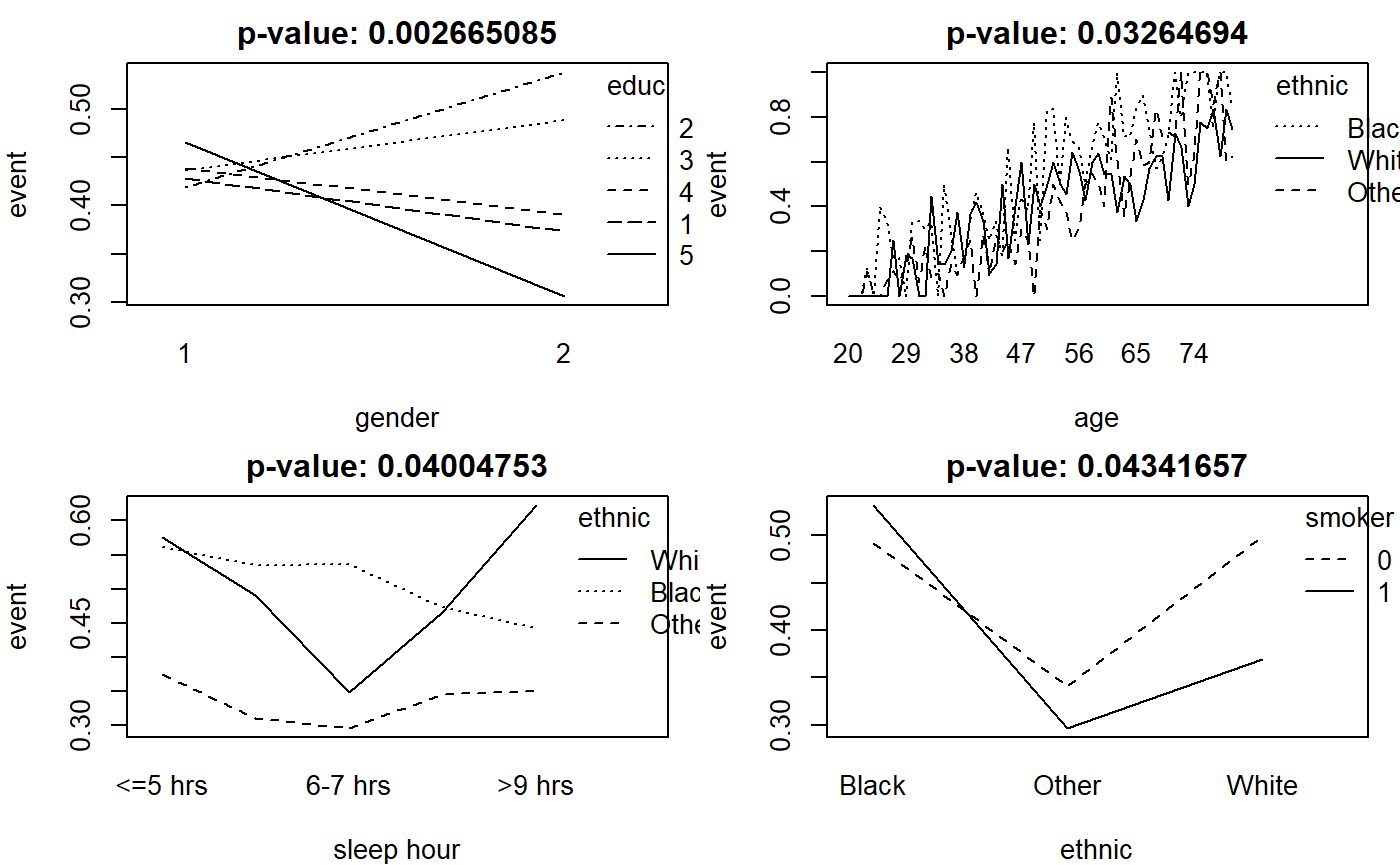
\includegraphics[width=0.9\textwidth]{Img/top4 interaction.png}
\caption{Two-Way Interaction Plots}
\end{figure}

Furthermore, we wrote an R function to utilize the LR test to test the significance of these interaction terms (see Table 3). The results suggest that the interaction between gender and education is a significant predictor ($<0.01$). Consequently, retaining the gender variable is warranted if we include the \verb|gender*education| interaction term. Therefore, we decided to keep all variables plus the interaction term \verb|gender*education| for our full model selection.


\begin{table}[!ht]
    \centering
    \small
    \caption{Interaction term p-value }
    \begin{tabular}{lllllllll}
    \hline
    \hline
        \textbf{} & \textbf{age} & \textbf{bmi} & \textbf{diabetes} & \textbf{educ} & \textbf{ethnic1} & \textbf{gender} & \textbf{sleep.hrs} & \textbf{smoker } \\ \hline
        \textbf{age} & ~ & 0.358 & 0.554 & 0.154 & 0.033* & 0.834 & 0.972 & 0.468  \\ \hline
        \textbf{bmi} & 0.358 & ~ & 0.097 & 0.314 & 0.679 & 0.496 & 0.399 & 0.912  \\ \hline
        \textbf{diabetes} & 0.554 & 0.097 & ~ & 0.206 & 0.05* & 0.38 & 0.74 & 0.293  \\ \hline
        \textbf{educ} & 0.154 & 0.314 & 0.206 & ~ & 0.849 & 0.003** & 0.729 & 0.583  \\ \hline
        \textbf{ethnic1} & 0.033* & 0.679 & 0.05* & 0.849 & ~ & 0.152 & 0.102 & 0.043*  \\ \hline
        \textbf{gender} & 0.834 & 0.496 & 0.38 & 0.003** & 0.152 & ~ & 0.184 & 0.106  \\ \hline
        \textbf{sleep.hrs} & 0.972 & 0.399 & 0.74 & 0.729 & 0.102 & 0.184 & ~ & 0.968  \\ \hline
        \textbf{smoker} & 0.468 & 0.912 & 0.293 & 0.583 & 0.043* & 0.106 & 0.968 &   \\ \hline
        \hline
    \end{tabular}
\end{table}

\newpage
For each categorical variable “gender”, “ethnic1” and “smoker”, we constructed a two-way table and a corresponding mosaic plot to evaluate their associations with cardiac events (Figure 3). According to the mosaic plots for binary variables “gender” and “smoker”, we find the proportion for two levels in each variable is nearly identical, and the dividing lines follow true for each level as well. From this plot, there is no visible association of these two variables. For the “Ethnic1”, we found the “Other” level has a significantly lower proportion of having cardiac events than other two ethnic. And since there is no obvious linear pattern, we kept all these three variables categorical.

\begin{figure}[!ht]
 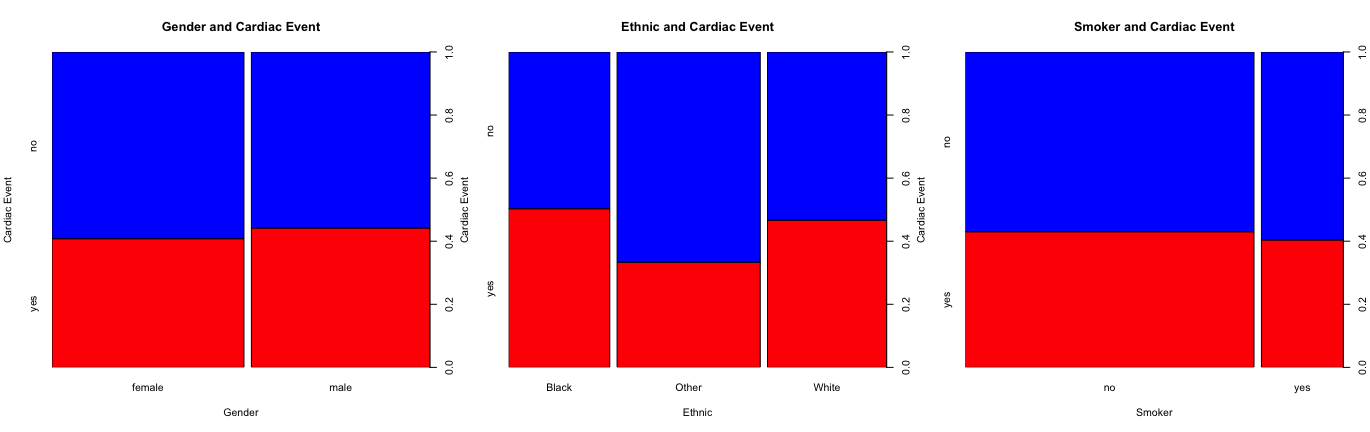
\includegraphics[width=\textwidth]{Img/moscia plot for categorical.png}
 \caption{Mosaic Plots for Gender, Ethnic, and Smoker}
\end{figure}

\newpage

In the “diabetes” mosaic plot (Figure 4 left), we can find there seems to be a linear relationship in three levels. The probability of getting a cardiac event is different for each level of diabetes status, and the probability seems to increase as the diabetes status becomes more severe. Using the tend test would confirm that diabetes status has a linear association with cardiac events (Figure 5). Based on the findings, we decided to keep the three distinct levels of diabetes status. We also re-coded the predictor, setting 1 (Yes) to 2, 2 (No) to 0, and 3 (Borderline) to 1, and set the predictor to continuous. After we removed the rows with missing diabetes status, we re-created the mosaic plot (Figure 4 right).

\begin{figure}[!ht]
\centering
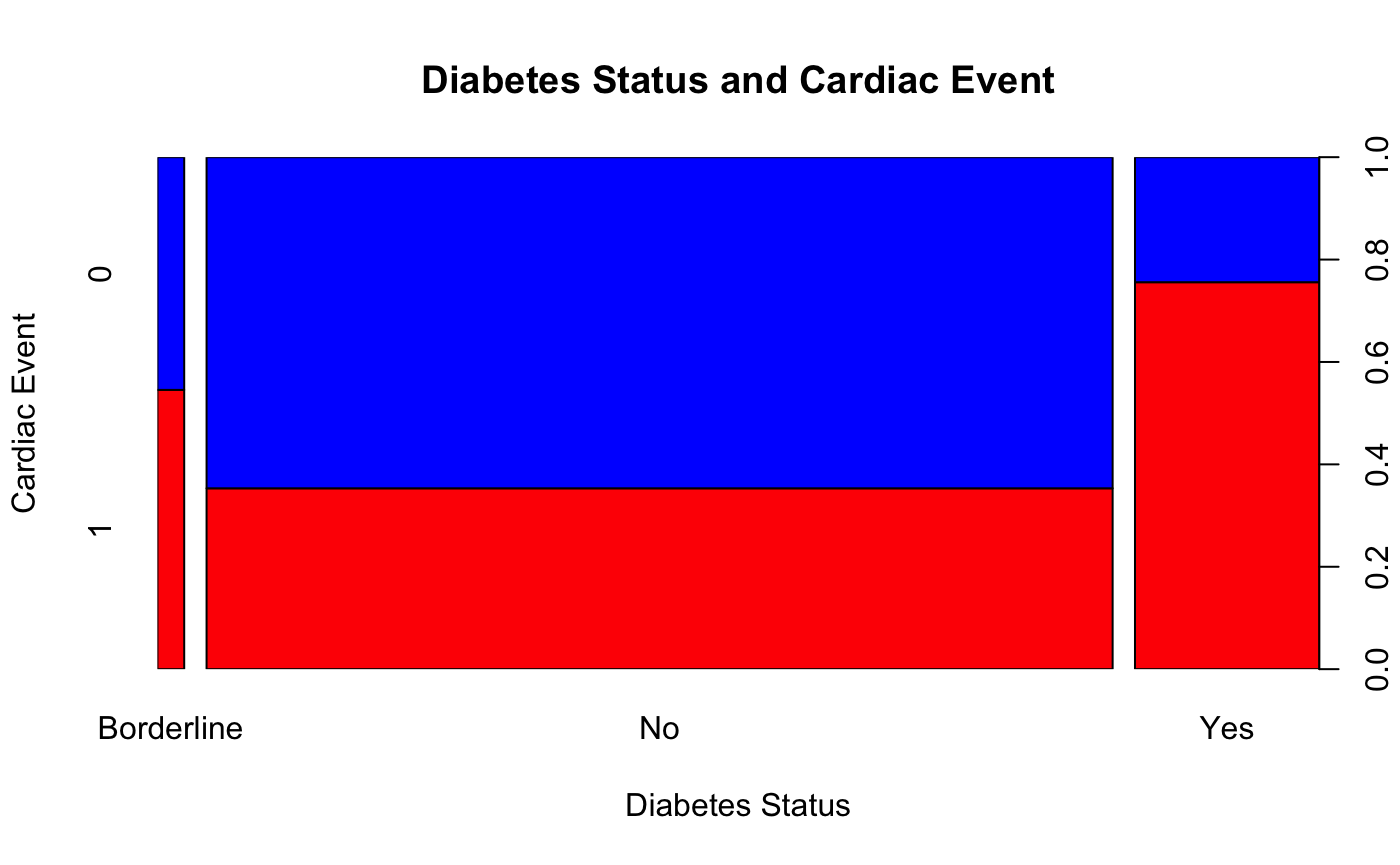
\includegraphics[width=0.4\linewidth]{Img/Diabetes Status and Cardiac Event.png}
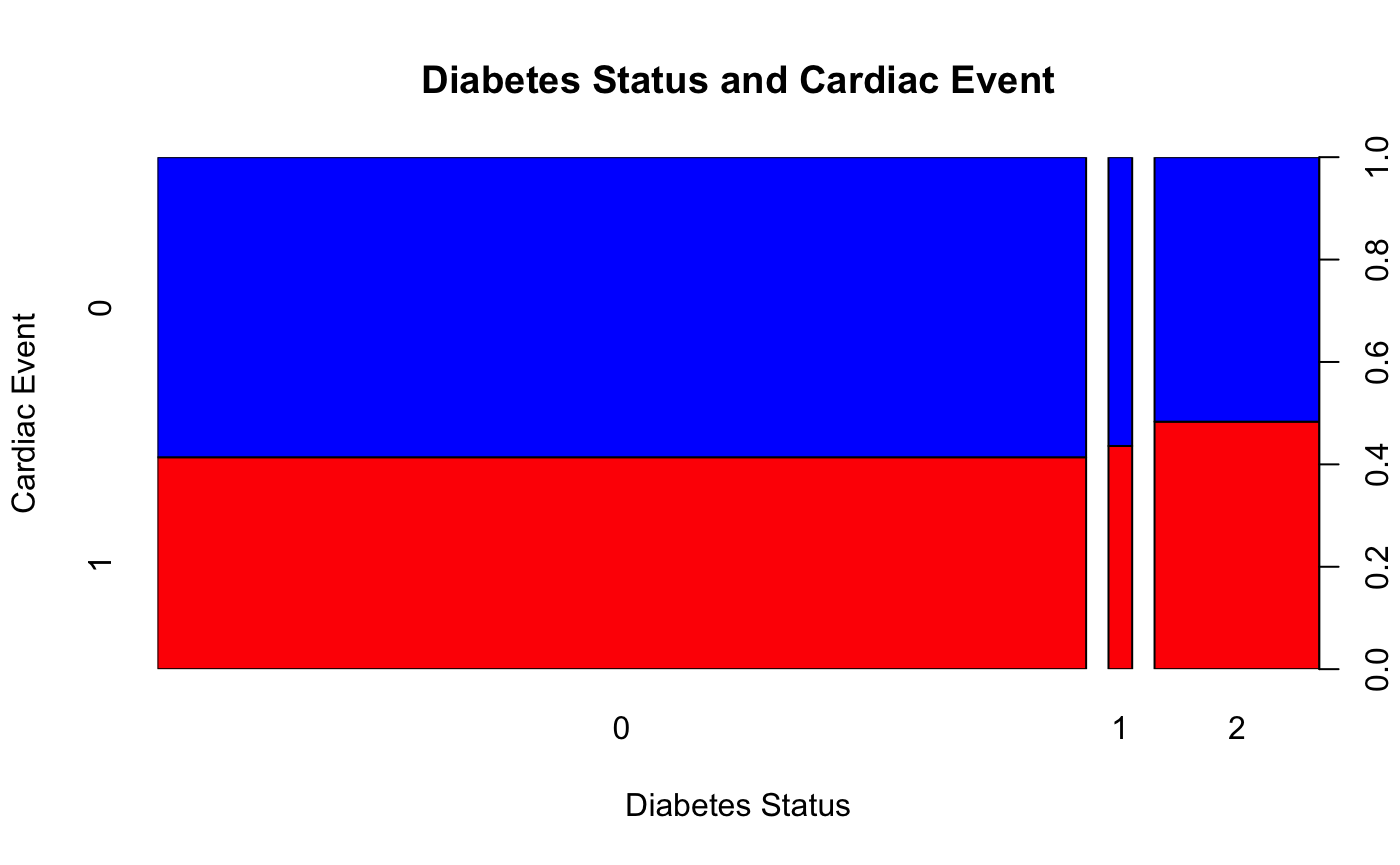
\includegraphics[width=0.4\linewidth]{Img/Diabetes Status and Cardiac Event Process.png}
\caption{Mosaic Plot for Diabetes}
\end{figure}

\begin{figure}[!ht]
\centering
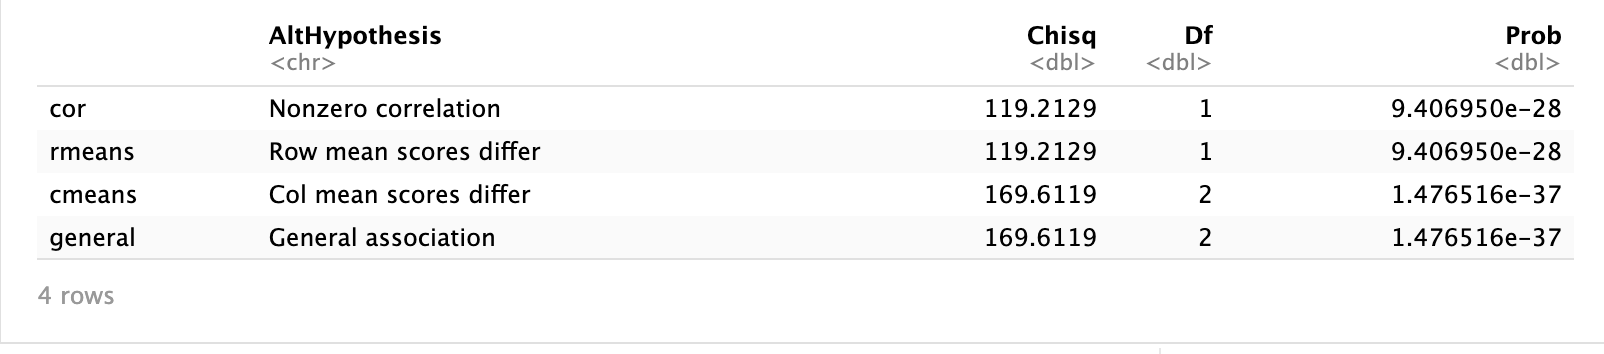
\includegraphics[width=\textwidth]{Img/diabetes CMHtest.png}
\caption{Trend Test Results for Diabetes}
\end{figure}
\newpage
For the numerical variables, “age” and “bmi”, we checked the relationship with the log-odds of success (experiencing cardiac event) using slicing. The slicing plots indicate that both variables have a roughly linear relationship with log odds (Figure 6). We can see that  as age and BMI increases, the log-odds of having cardiac events also increases. The linear pattern serves as evidence to us that the two variables do not require any transformation. Thus, we decided to keep age and BMI as numerical variables, without any transformation.

\begin{figure}[!ht]
\centering
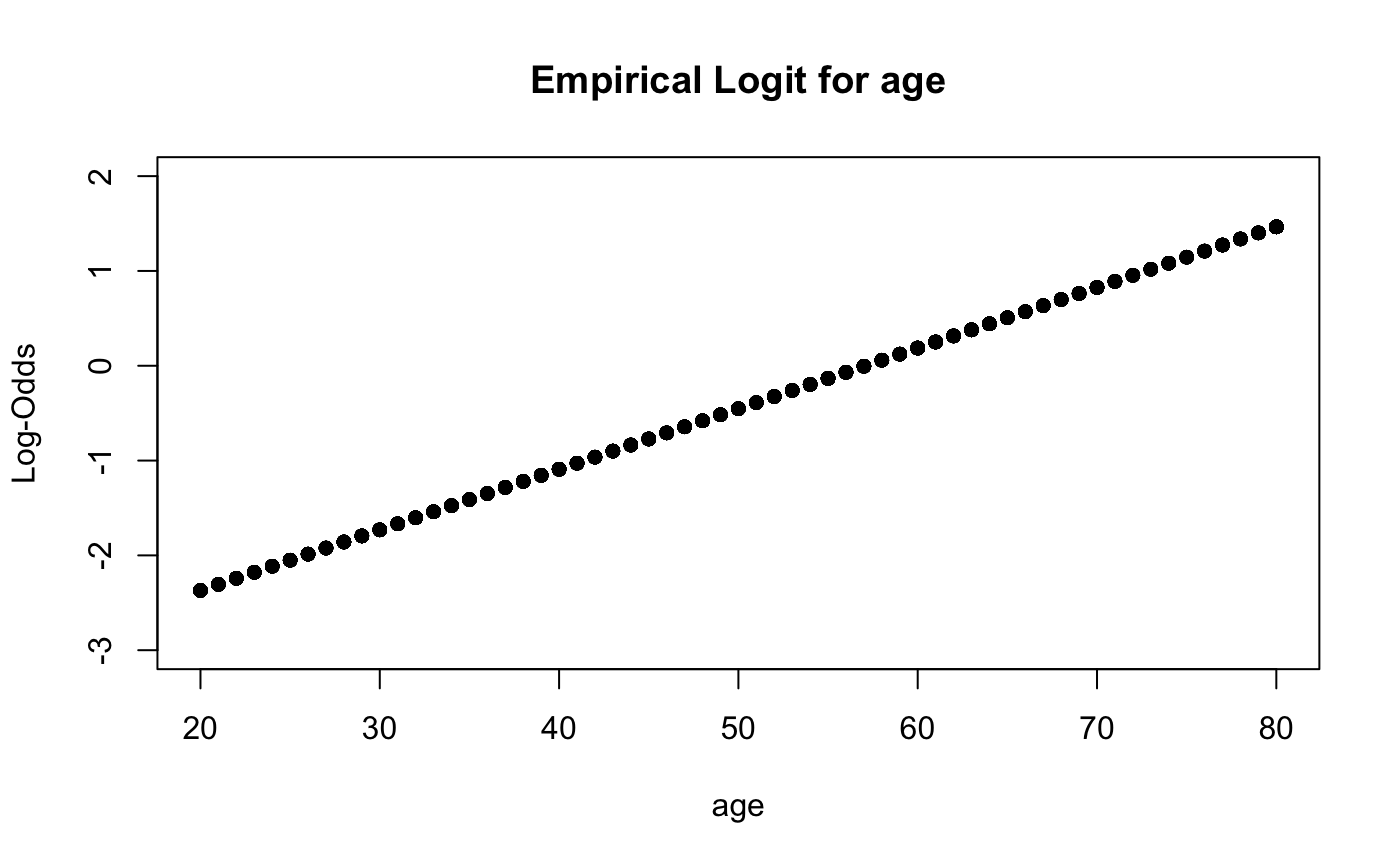
\includegraphics[width=0.45\textwidth]{Img/Empirical Logit for Age.png}
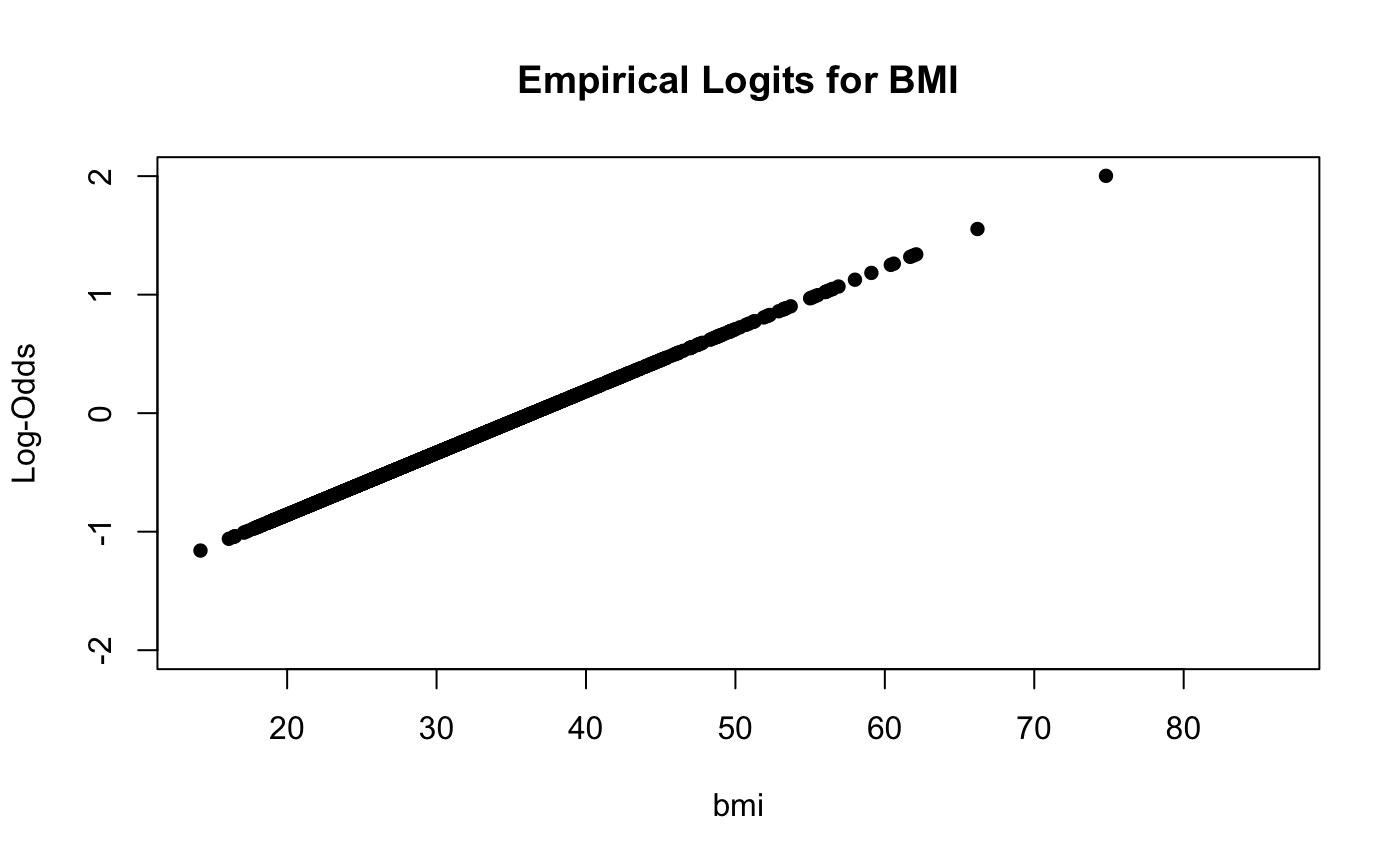
\includegraphics[width=0.45\textwidth]{Img/Empirical Logits for BMI.png}
\caption{Slicing Plots for Age and BMI}
\end{figure}

During the data cleaning phase, we can see that the observations for sleep hour are very dispersed (Figure 7 histogram). Some hours have many observations, while some only have few. Therefore, we decided to recombine the observations. Since the number of observations for over 9 hours and less than 5 hours are very few, we combined the observations at the two extremes to separate groups. We then created the mosaic and slicing plot, and discovered that the sleep hours between 7-8 hrs and 8-9 hrs have the same level (people in the two groups have around the same probability of experiencing cardiac events). Therefore, we combined these two groups together and recreated the mosaic plot. After we re-categorized the sleep hour variable, we ended up with five categories: “<=5 hrs”, “5-6 hrs”, “6-7 hrs”, “7-9 hrs” and “>9 hrs”. Furthermore, the trend test (Figure 8) shows no obvious linear relationship between sleep and experiencing cardiac events, so combining categories would not have significant impacts on the results of our data analysis.

\begin{figure}[!ht]
\centering
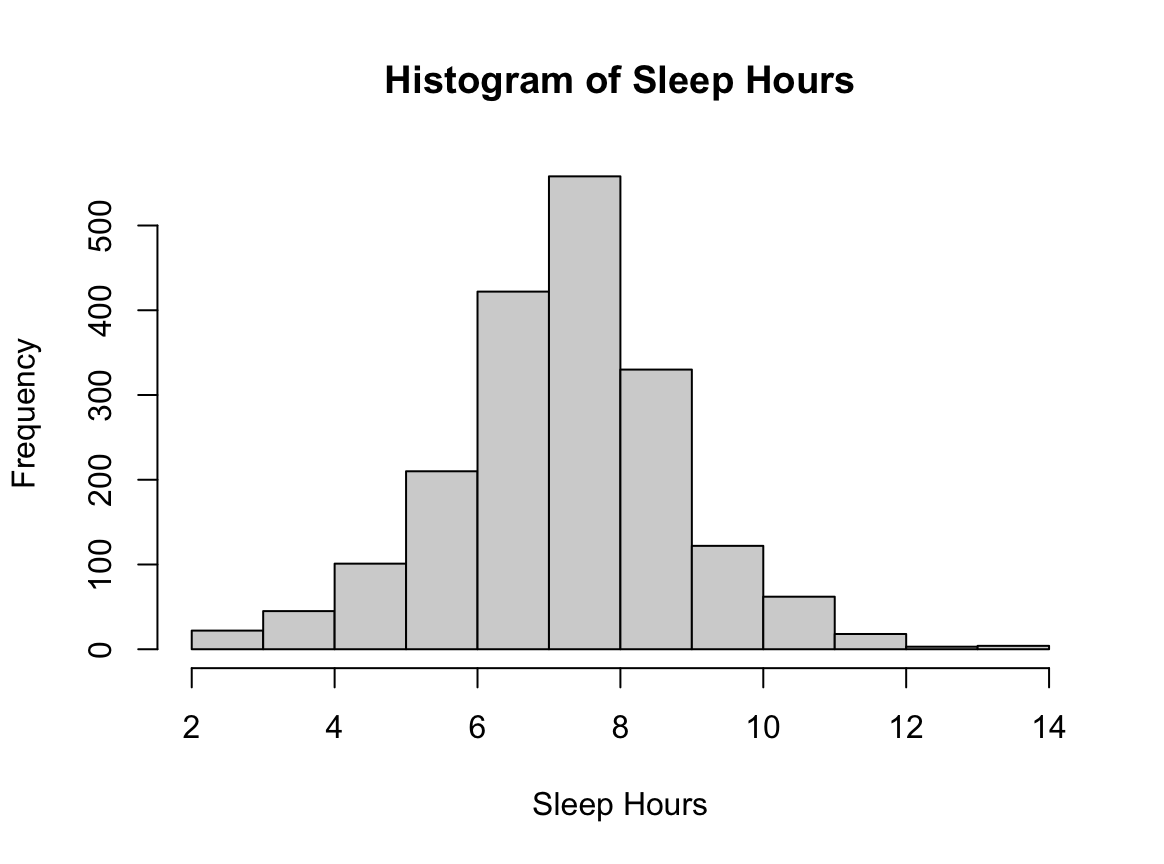
\includegraphics[width=0.3\textwidth]{Img/hist of sleep hours.png}
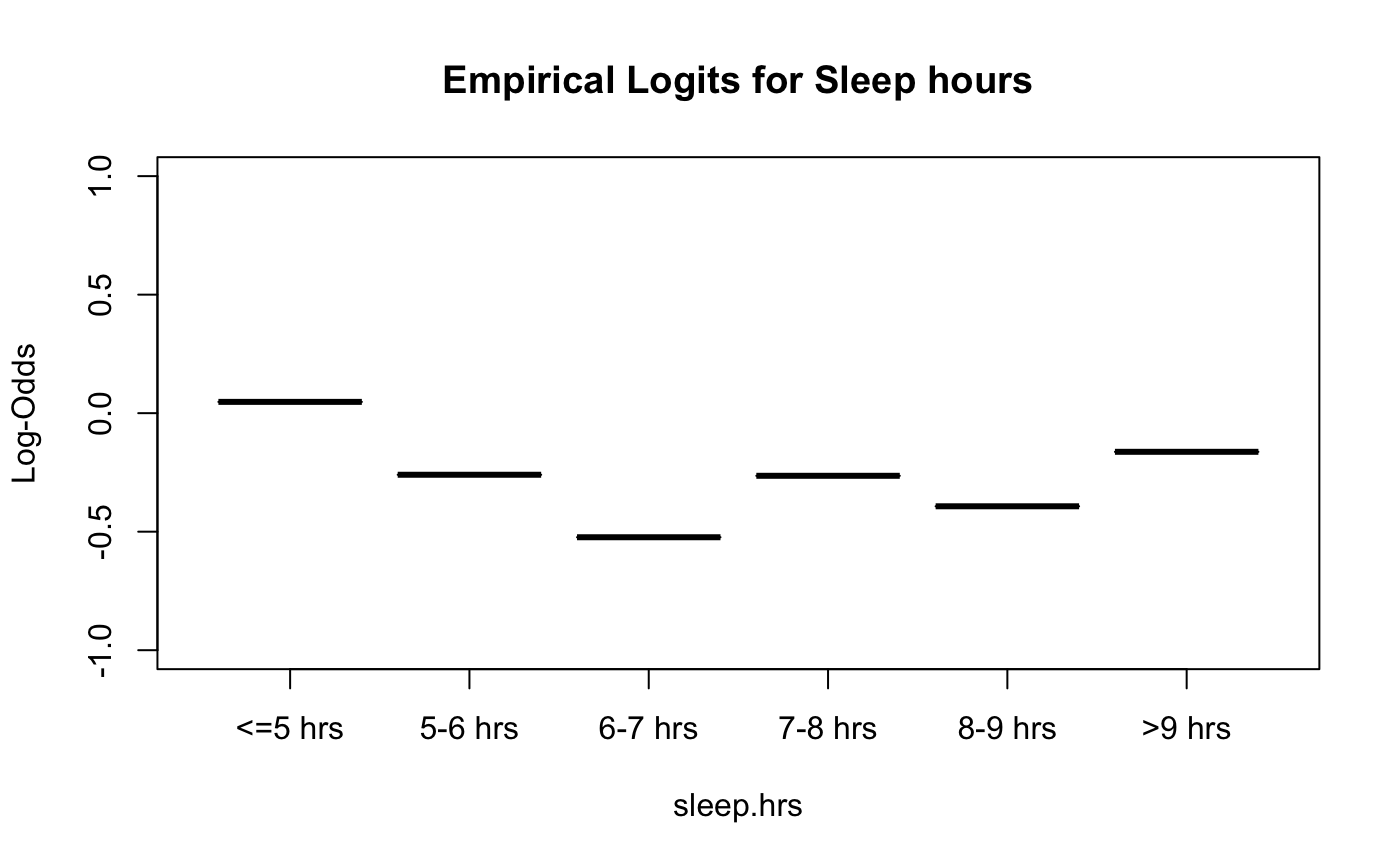
\includegraphics[width=0.3\textwidth]{Img/Empirical mid for sleep.png}
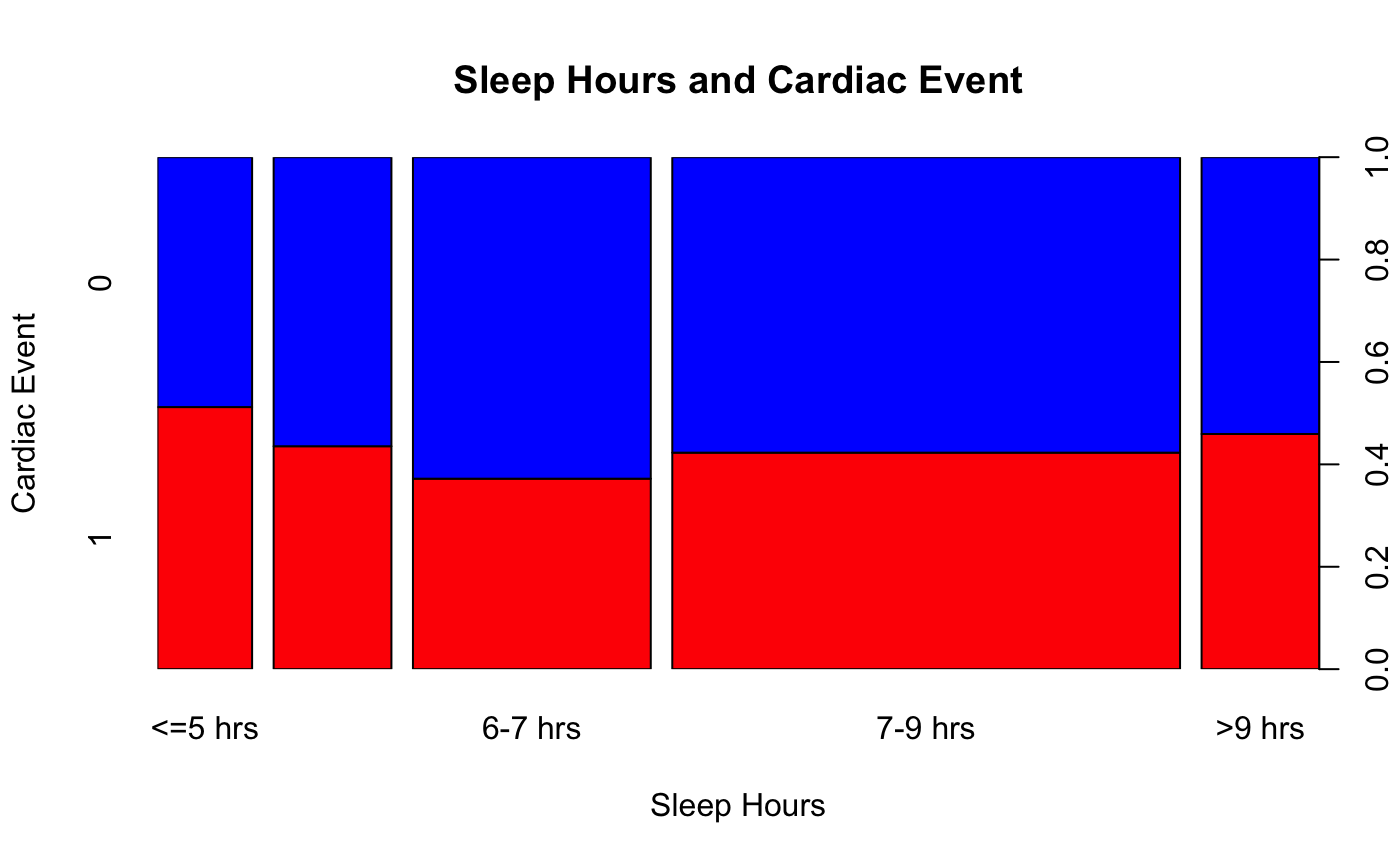
\includegraphics[width=0.3\textwidth]{Img/Sleep Hour and Cardiac Event.png}
\caption{Histogram and Mosaic for Sleep Hours}
\end{figure}

\begin{figure}[!ht]
    \centering
    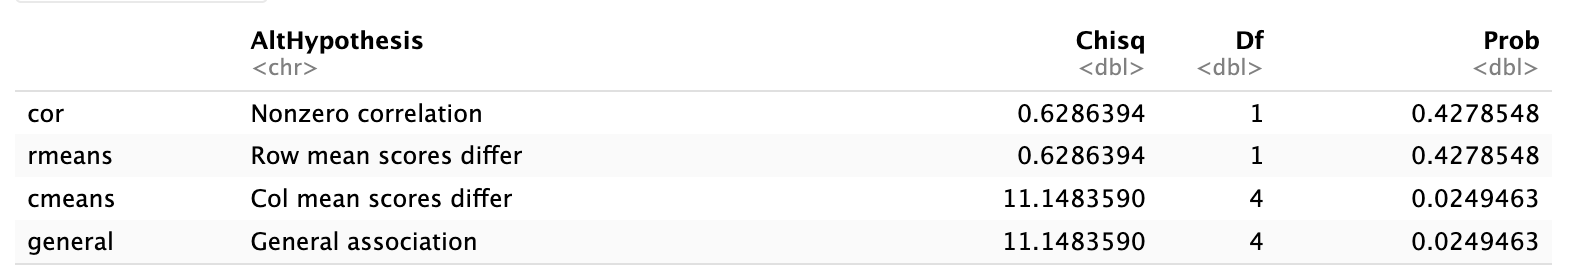
\includegraphics[width=\textwidth]{Img/sleep CMHtest.png}
    \caption{Trend Test Results for Sleep Hours}
\end{figure}

% Model Selection: Multivariate Analysis Using Logistic Model

\subsection*{Model selection }
Having variables from the procedures above, we use the model with all 8 variables and the significant interaction term (gender*educ) as the starting model to select our final model from a backward selection process using the function called \verb|step()| in R. For the candidates model, we obtain both the AIC, BIC, and their p value for comparison and form them into a table.

% ^, where p-value($\sim$null) is calculated from the $G^2_{\text{null}}-G^2_{\text{residual}} \sim  \chi ^2 _{df_\text{null}-df_\text{residual}}$ and p-value($\sim$full) is calculated from $G^2_{\text{residual}} \sim  \chi ^2 _{df_\text{residual}}$
% refers to significance of the model being different with the full model:

\begin{table}[!ht]
\caption{Model selection (Null Deviance|df=2503.0|1835)}
    \centering
    \small
    \begin{tabular}{lllllll}
    \hline
    \hline
        \textbf{Predictors} & \textbf{Residual Dev.} & \textbf{df} & \textbf{p-value($\sim$null)} & \textbf{p-value($\sim$full)} & \textbf{AIC} & \textbf{BIC} \\ \hline
        G,A,Et,Ed,Sl,D,Sm,B,Ed*G & 1907.2 & 1816 & <0.0001 & 0.069 & 1947.17 & 2057.48  \\ \hline
        G,A,Et,Ed,D,Sm,B,Ed*G & 1911.7 & 1820 & <0.0001 & 0.066 & \textcolor{pink}{\textbf{1943.66}} & 2031.91  \\ \hline
        G,A,Et,Ed,D,Sm,B & 1919.7 & 1824 & <0.0001 & 0.058 & \textcolor{pink}{\textbf{1943.66}} & 2009.85  \\ \hline
        G,A,Et,D,Sm,B & 1927.6 & 1828 & <0.0001 & 0.052 & \textcolor{pink}{\textbf{1943.6}} & 1987.67  \\ \hline
        A,Et,Ed,D,Sm,B & 1921 & 1825 & <0.0001 & 0.058 & \textcolor{pink}{\textbf{1942.96}} & 2003.63  \\ \hline
        A,Et,D,Sm,B & 1928.8 & 1829 & <0.0001 & 0.051 & \textcolor{pink}{\textbf{1942.79}} & 1981.39  \\ \hline
        A,Et,Sm,B & 1932.2 & 1830 & <0.0001 & 0.047 & \textcolor{pink}{\textbf{1944.22}} & \textcolor{red}{1977.31}  \\ \hline
        A,Et,B & 1938 & 1831 & <0.0001 & 0.04 & 1948.02 & 1975.6  \\ \hline
        \hline
    \end{tabular}
\end{table}



In the table above, predictors are the abbreviations of the first one or two starting letters of each variable, whereas asterisks represent interaction terms. Compared with the null model, all the candidates have significant p-values. With the minimum AIC being 1942.79, this comes from the model obtained from predictors A,Et,D,Sm, and B. For accuracy, we also treat models with AIC value of $\min{\text{AIC}} \pm 2$ as optimal models (in pink). \\

Based on this criteria, we further filter out all models except for the one with exact minimal BIC values (in red), which is the model with predictors A,Et,Sm,B. Our final model is in the following form:

{\small
\begin{align*}
\text{logit}(\pi_E)=\ln  \left( \frac{\mathbb{P}(\text{event})}{1-\mathbb{P}(\text{event})} \right)&=\beta_0+ \beta_{\text{age}} \text{age}+ \beta_{\text{Ethnic:Other}} \text{Ethnic:Other} \\
&+\beta_{\text{Ethnic:White}} \text{Ethnic:White}
+\beta_{\text{Ethnic:White}} \text{Ethnic:White}+\beta_{\text{Smoker}} \text{Smoker} + \beta_{\text{BMI}} \text{BMI}
\end{align*}
}%

In order to have a more comprehensive overlook of the model, the following table 6 gives the point estimates of coefficients, odds ratio, and their 95\% confidence intervals along with the p-values for the coefficients:

\begin{table}[!ht]
\caption{Statistics of variables in the final model}
    \centering
    \begin{tabular}{lllll}
    \hline
    \hline
        \textbf{Predictor}  & \textbf{Parameter estimates}  & \textbf{Odds ratios}  & \textbf{Odds ratio CI}  & \textbf{p-value} \\ \hline
        (Intercept) & -5.84 & 0.0029 & [0.0014,0.0060] & <0.0001 \\ \hline
        age & 0.073 & 1.08 & [1.07,1.08] & <0.0001 \\ \hline
        ethnic1:Other & -0.59 & 0.554 & [0.423,0.731] & <0.0001 \\ \hline
        ethnic1:White & -0.63 & 0.533 & [0.399,0.707] & <0.0001 \\ \hline
        smoker1 & 0.33 & 1.39 & [1.06,1.83] & 0.0161 \\ \hline
        bmi & 0.067 & 1.07 & [1.05,1.09] & <0.0001 \\ \hline
        \hline
    \end{tabular}
\end{table}
Our final model with fitted coefficient is then:
{\small
\begin{align*}
\text{logit}(\pi_E)=\ln  \left( \frac{\mathbb{P}(\text{event})}{1-\mathbb{P}(\text{event})} \right)&=-5.84+ 0.073 \text{age}-0.59 \text{Ethnic:Other} \\
&-0.63\text{Ethnic:White}
+0.33\text{Ethnic:White}+\beta_{\text{Smoker}} \text{Smoker} + 0.067 \text{BMI}
\end{align*}
}%

We then utilize the ROC curve to evaluate our model performance. It is commonly used to evaluate the performance of a binary classification model. The ROC curve shows that our model achieved a high performance in predicting cardiac events. Its AUC value of 0.808 indicates reliable performance (better than random guessing).



\begin{figure}[!ht]
\centering
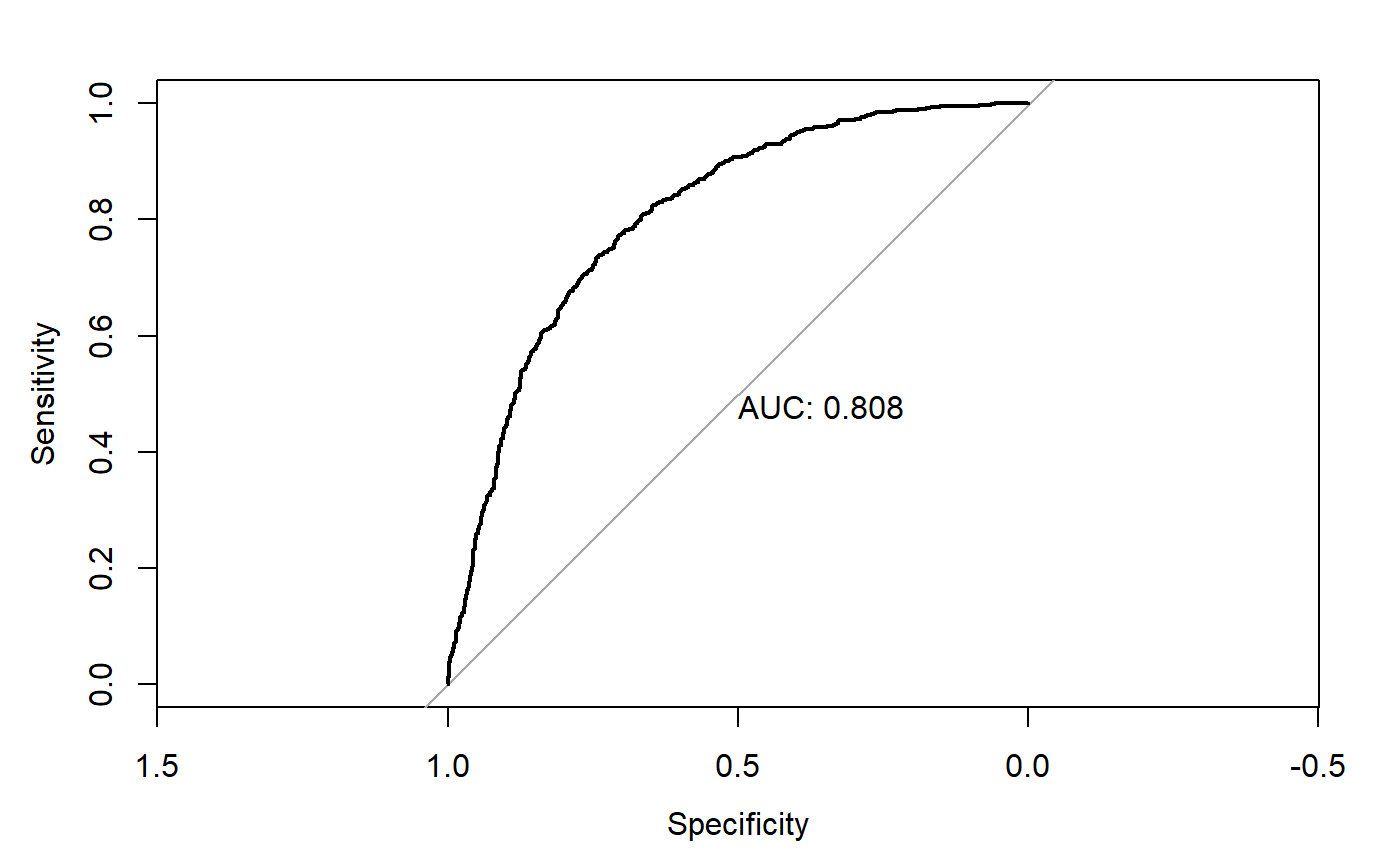
\includegraphics[width=0.5\textwidth]{Img/roc.png}
\caption{ROC curve plot}
\end{figure}

We cross-tabulate the true class labels against the predicted labels to make a confusion matrix. Based on the results generated above, our model made correct predictions for 833 patients who did not have heart disease (true negatives) and 527 patients who did have the disease (true positives). This means that our model has an accuracy of 74.07\% (1360/1836). Meanwhile, it misclassified 252 patients without cardiac events as positive (false positives) and 224 patients with cardiac events as negative (false negatives), contributing an error rate of 25.93\% (476/1836).

\begin{table}[!ht]
\caption{Confusion matrix}
    \centering
    \begin{tabular}{|l|l|l|}
    \hline
        $_{\text{Prediction} }$ $\backslash$ $^{\text{Reference}}$  & \textbf{0(No)} &\textbf{ 1(Yes)}  \\ \hline
        \textbf{0(No) }& 833 (True negative) & 224 (False negative, Type II Error)  \\ \hline
        \textbf{1(Yes)} & 252 (False positive, Type I Error) & 527 (True positive)  \\ \hline
    \end{tabular}
\end{table}

% \pagebreak
% ^NEED FINAL CHANGE^ 
\newpage
Since our final model contains two continuous variables and two categorical variables, for the probability plots, we plotted a total of four pictures using the two continuous variables as the x-axis and correspond to the two categorical variables, respectively.


\begin{figure}[!ht]
    \centering
    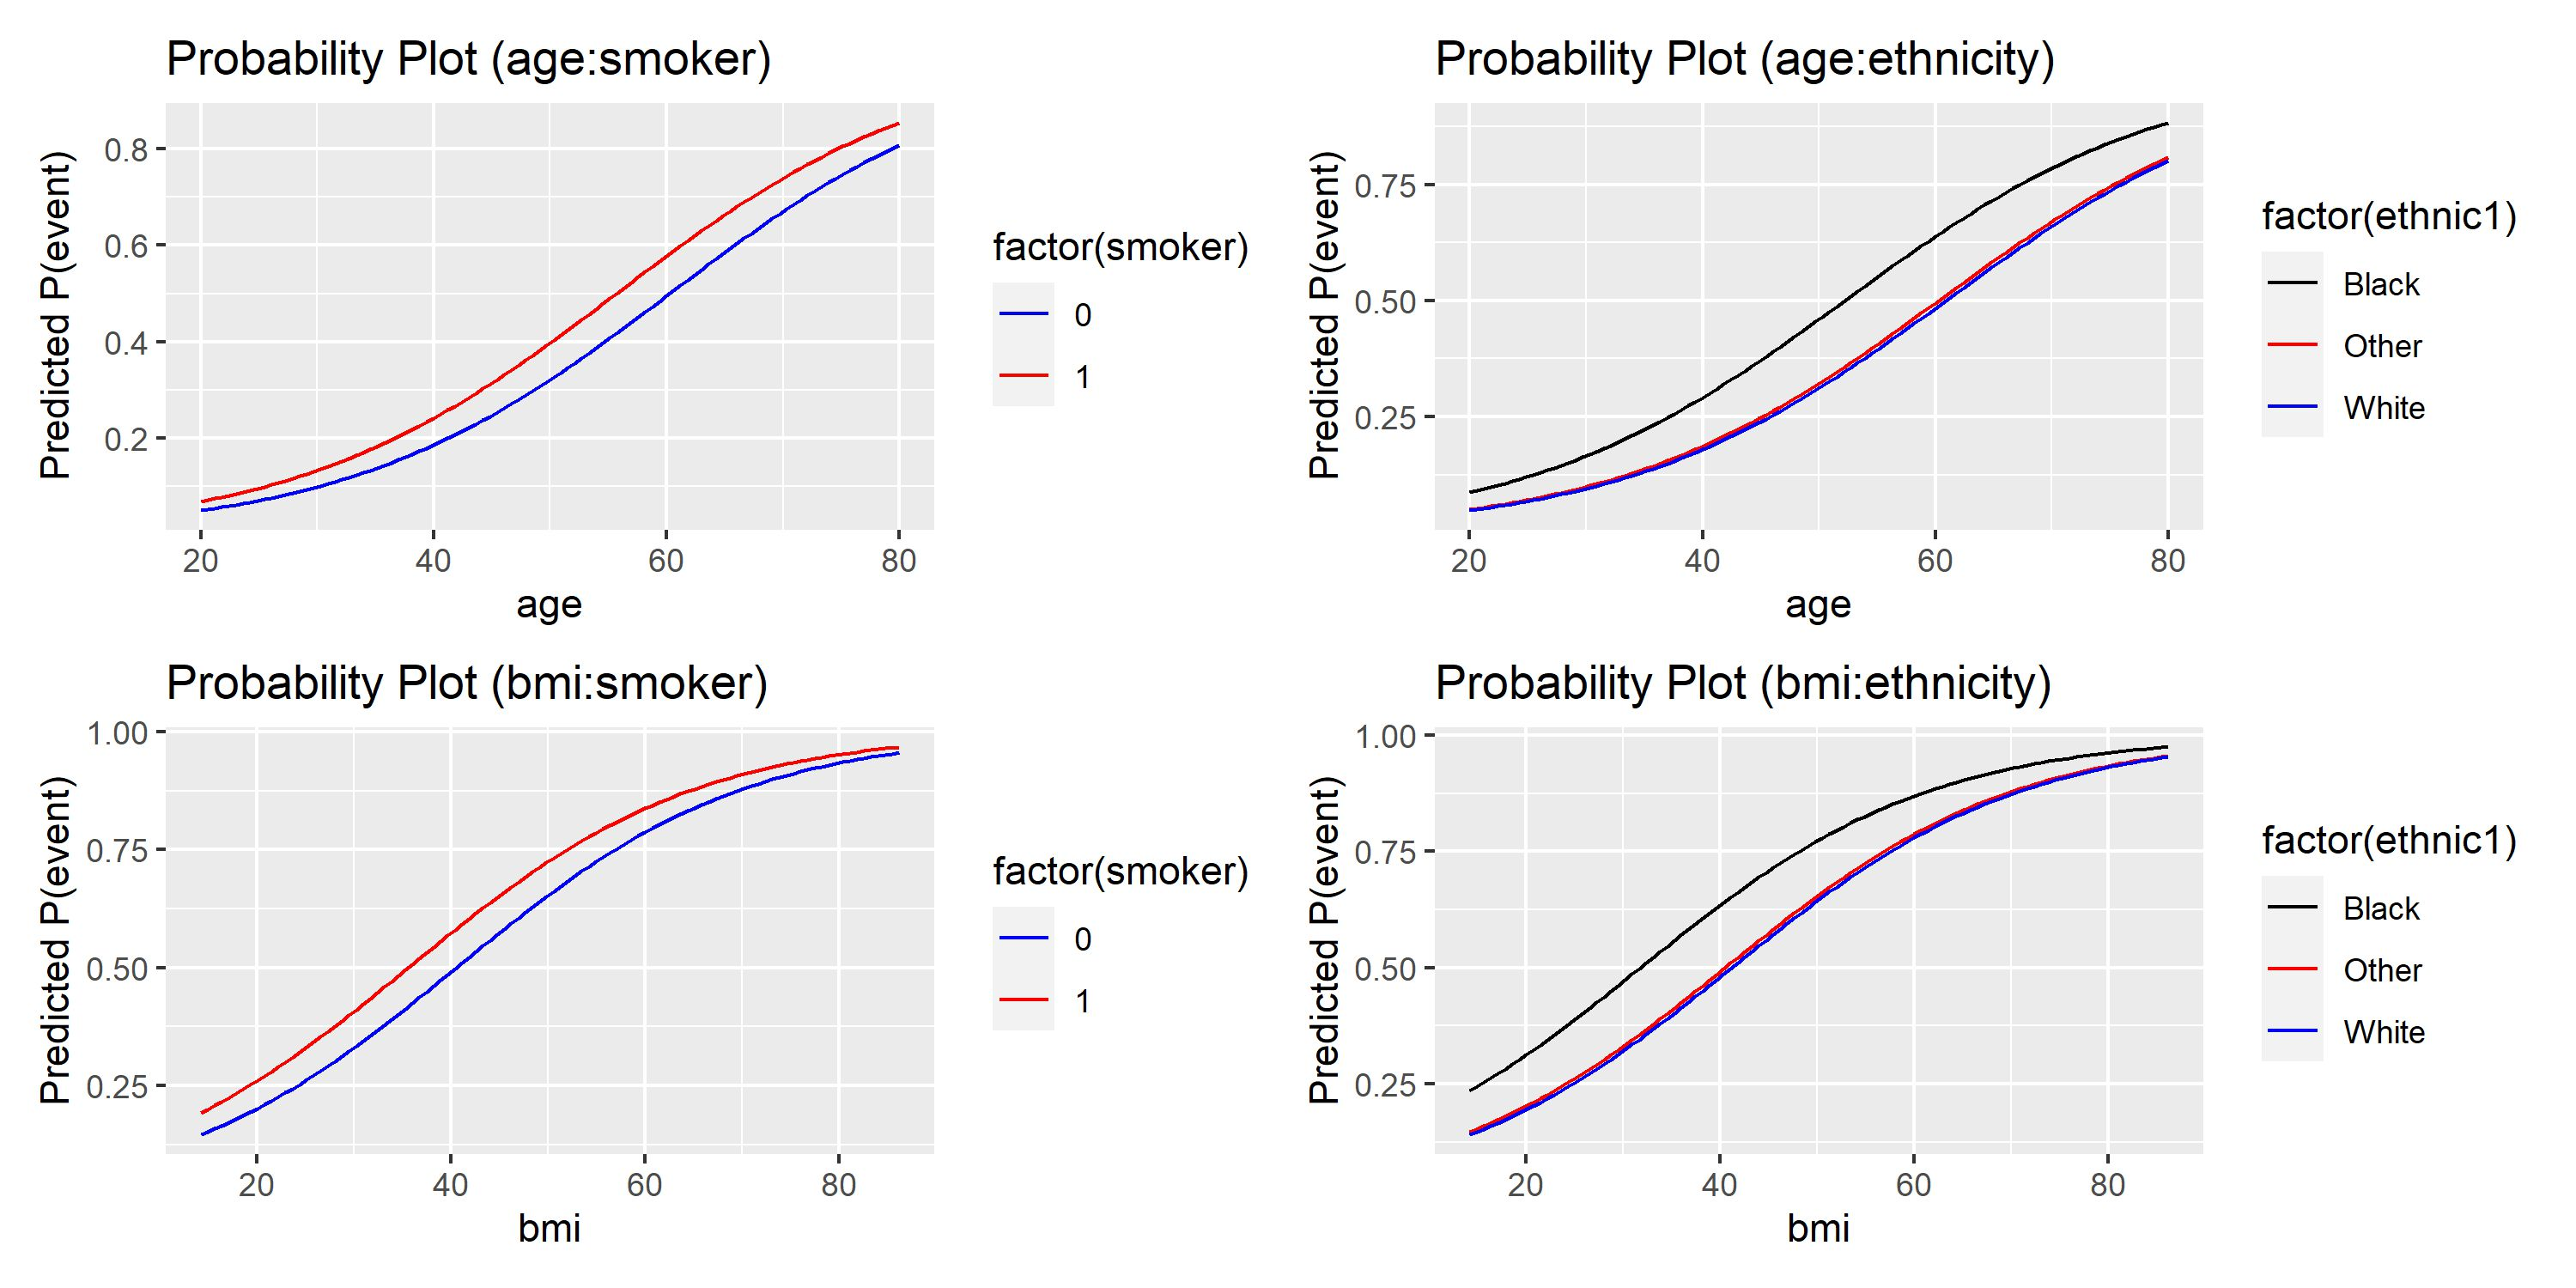
\includegraphics[width=\textwidth]{Img/prob_plot.jpg}
    \caption{Probability Plot for Significant Variables}
\end{figure}


For each plot, we changed the value of the continuous variables to analyze how different classifications in the categorical variables affected predicted results according to our final model while controlling the other 2 variables constant to be the mean (continuous) or the most common value (categorical) of its group. For the two graphs on the left, we can see that while controlling for either age or BMI, the smoker group has a higher predicted probability of getting cardiac diseases, compared to non-smokers. For the two graphs to the right, we can see that through controlling for age or BMI, black-identifying individuals from the ethnicity category have a higher probability of cardiac disease. The other two ethnic groups (white and others) have roughly the same predicted probability of cardiac disease when controlling for age or BMI as well. To elaborate, age has a larger effect on the probability of having a heart disease; as illustrated by the graphs in the first row curving upwards while gradually diverging as age increases. Whereas BMI is the opposite. Curves in the second rows converge, indicating a smaller effect on the probability of having a heart disease as BMI goes up.


\section*{Discussion}
Our final model includes age, ethnic, smoker, and BMI as significant predictors for cardiac events. It is important to understand the effect and direction of each of the predictors in the model. In order to contextualize and give meaning to the effect and direction of each predictor, we will use odds ratios. 
\subsection*{Age}
The predictor “age” has a moderate influence on the probability of developing cardiac diseases. Following the model, it appears that for every one year increase in age (holding all other variables constant), the odds of the cardiac event occurring increase by approximately 8\% (exp(0.073)). In simpler terms, as people get older, the likelihood of getting cardiac disease increases by around 8\%.

\subsection*{Ethnicity}
The predictor “ethnic” was treated as a categorical variable in our model, and we represented it through dummy coding. According to the model, both the “white ethnic” and the “other ethnic” have a negative relationship with the odds of having cardiac events. This means that people belonging to the “black ethnic” group have greater odds of developing cardiac diseases. Compared to the “white ethnic” group, the odds for developing cardiac diseases is around 87.6\% higher (inverse of the odds ratio for ethnic:white) for the  “black ethnic” group. Compared to the “other ethnic” group, the odds for developing cardiac diseases is around 80.5\% higher (inverse of the odds ratio for ethnic:other) for the  “black ethnic” group.

\subsection*{Smoker}
Furthermore, smoking status is also identified as a significant predictor. Based on the results in Table 5, we can see that the odds of getting cardiac diseases increases by around 39\% for smokers (holding all other variables constant). This result implies that smoking is linked to a notable increase in the development of cardiac events.

\subsection*{BMI}
Lastly, body mass index (BMI) demonstrates a significant positive effect on the event. For every one-unit increase in BMI, the odds of having a cardiac event increase by approximately 7\% (holding all other variables constant), indicating that higher BMI is associated with a significant rise in the likelihood of developing cardiac events.

\subsection*{Notes on Sleep Hours}
Our model selection analysis determined that the duration of one’s sleep did not have an effect on the cardiac arrest event. As we discussed in the results section, we decided to treat sleep as a categorical variable instead of continuous due to the results from the splicing plot. The Chi-square test of association also shows that the amount of sleep is not associated with the development of cardiac events, but we still include it during the model selection process. During model selection, we ran backward selection twice, using both AIC and BIC as evaluating criteria, and the results show that sleep hour is the first variable being dropped out from the model. The model performance had a noticeable improvement after dropping this predictor. Thus, we conclude that nightly sleep hours don't affect the chance of developing cardiac diseases.

\subsection*{Problems encountered during the analysis}
The first problem we encountered was handling the missing values. Due to the large amount of missing values, we ran regression models to predict missing values. However, the diabetes variables have three ordinal outcomes. Multinomial logistic regression is out of the scope of our analysis, so we have to delete all the rows with missing diabetes status.\\
The second problem we encountered was classifying variable types and re-coding categorical variables for analysis. We utilized the splicing plot to determine the variable type. As for re-coding the categorical variables, we used a trend test and mosaic plot to help us determine if we need to combine distinct categories.\\
During our model selection phase, we realized that many of the models we generated had very close AIC for comparison purposes. While we wanted to prioritize goodness of fit, we quantified another metric to select potential predictors, the BIC. The BIC allowed us to select variables that fit the model with the best subset to prioritize the precision and accuracy of the model’s predictive abilities. 

	
\subsection*{Further research}

Further research on this subject could explore more predictors of cardiac events at patient level. According to the American Heart Association, individuals with arrhythmia already experience unusual contractions of heart activity. Data on whether the patient already experiences an irregular blood flow could provide valuable information on predicting cardiac events. Due to the nature and severity of cardiac events, given more time, we would have aimed to improve the power of our model and minimize the probability of encountering a false negative (incorrectly deeming someone at risk for cardiac failure healthy).


It could also be interesting to investigate whether a prior history of cardiac events occurring within the family has an impact on patient health. Introducing this factor into the project could reveal potential genetic or hereditary influences on patient health already studied here, such as if certain ethnicities are more prone to diabetes than others. In the same vein, we noticed in this study that while not incredibly high, smoking and age were somewhat correlated. Since these predictors were significant in our final model, further analysis could be valuable in determining appropriate intervention for this group. 


% \newpage 
% \section*{\textit{DRAFT ZONE:}}


\end{document}